\section{Model 1:Fungi Population Prediction Model}
		\subsection{Competitive Lotca-Voterra Equations}
        We assume that there is only one kind of fungi, Phlebia acerina DR60 A8A,and using data as follows:
\begin{align}%单位改正体,下同
    T=22^{\circ}C,M=-0.5\text{MPa},n=0.97,v_{\text{ex}}=8.51\text{mm/day},\nonumber\\
    \rho_{hy}=0.27\mu g/cm^2,v_{de}=73.39\pm 10.22\%/122\text{days}\nonumber
\end{align}



where r is pamrameter of describing the speed of growth, and k is bioligical capacity.

We assume that there are N kinds of different fungi, and the biomass of each kind of fungi is $S_i$. We only concern about the relative biomass of each kind of fungi, so we substitute $S_i$ with $x_i=S_i/K_i$.

We use the Competitive Lotca-Voterre equations, a model for the population dynamics of species competing for some resource. 

\begin{align}
    \frac{dS_i}{dt}=r_i S_i  (1- \frac{\sum_{j=1}^{N}\alpha_{ij}S_j}{K_i})
\end{align}

Using the substitution $x_i=S_i/K_i$, the equations can be written as below:

\begin{align}
    \frac{dx_i}{dt}=r_i x_i  (1- \frac{\sum_{j=1}^{N}\alpha_{ij}x_jK_j}{K_i})
\end{align}

where
\begin{align}
    r_i&=\frac{v_{extension}}{R}\\
    K_i&=C\rho_i,C=const\\
    \alpha_{ij}&=\exp{1-\frac{n_i}{n_j}}\\
    \epsilon&=0.33
\end{align}

$\epsilon\:$is efficiency, according to the reference[3].
		\subsection{Parameter Estimation of LV Equations}
        We assume that $\alpha_{ij}=\exp(1-n_i/n_j)$, making the fungi with larger n having advantages over fungi with smaller n.
			\subsubsection{Carrying Capacity:K}
			\subsubsection{Inherent Per-capita Growth Rate:r}
            When there's only one kind of fungi, it evolve as he equation below:

            \begin{align}
                \frac{dx(t)}{dt}=r(T,M)x(t)(1-\frac{S(t)}{K(T,M)})
            \end{align}
            So we assume that $r=\left< \frac{dS}{dt} \right>$
		\subsection{Results}
        We choose several kinds of fungi, the data are shown as follow:

and the result after enough long time of evolution is shown in Figure 1, where temperature $T=25^{\circ}C$, moisture $M=-0.5MPa$

\begin{figure}[H]
    \centering
    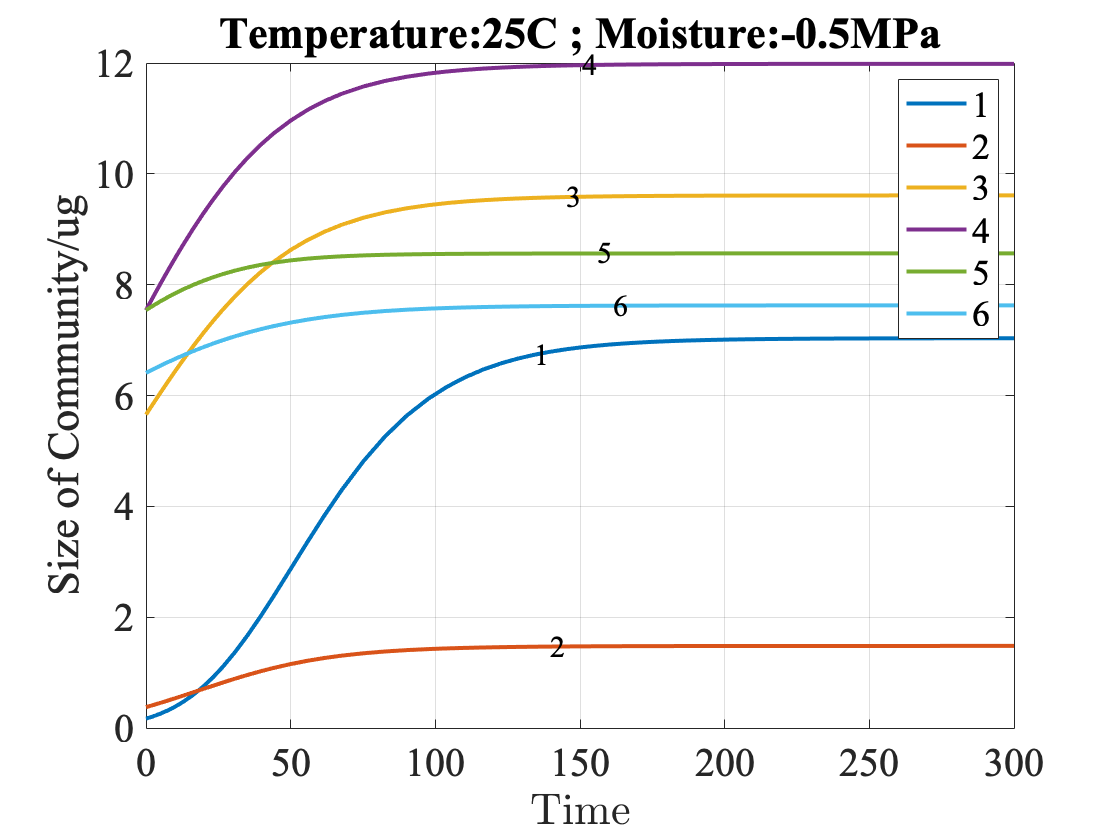
\includegraphics[width=.6\textwidth]{25_05.png}
    \caption{The result of Model 1}\label{fig:result1}%引用标记
    \end{figure}

%---------------------------------------------			
	\subsection{Detail 1 about Model 1}

%-------------------------------------------------







